\documentclass[english, a4paper]{article}
\author{Kim Rune Solstad}
\title{TDT4136, Assignment 6}
\usepackage{graphicx}
\usepackage{amsmath}

\begin{document}

\maketitle
\section{Planning Graph}
Negations has been ignored in this graph, as most of the conditions will function as negations. Assumptions that the agent is able to do more than one task has been made. That is why the plannin graph is non-serial. Also, the graph is not expanded until the graph has leveled-off. This is because a solution was found before such a point was reached.
\\
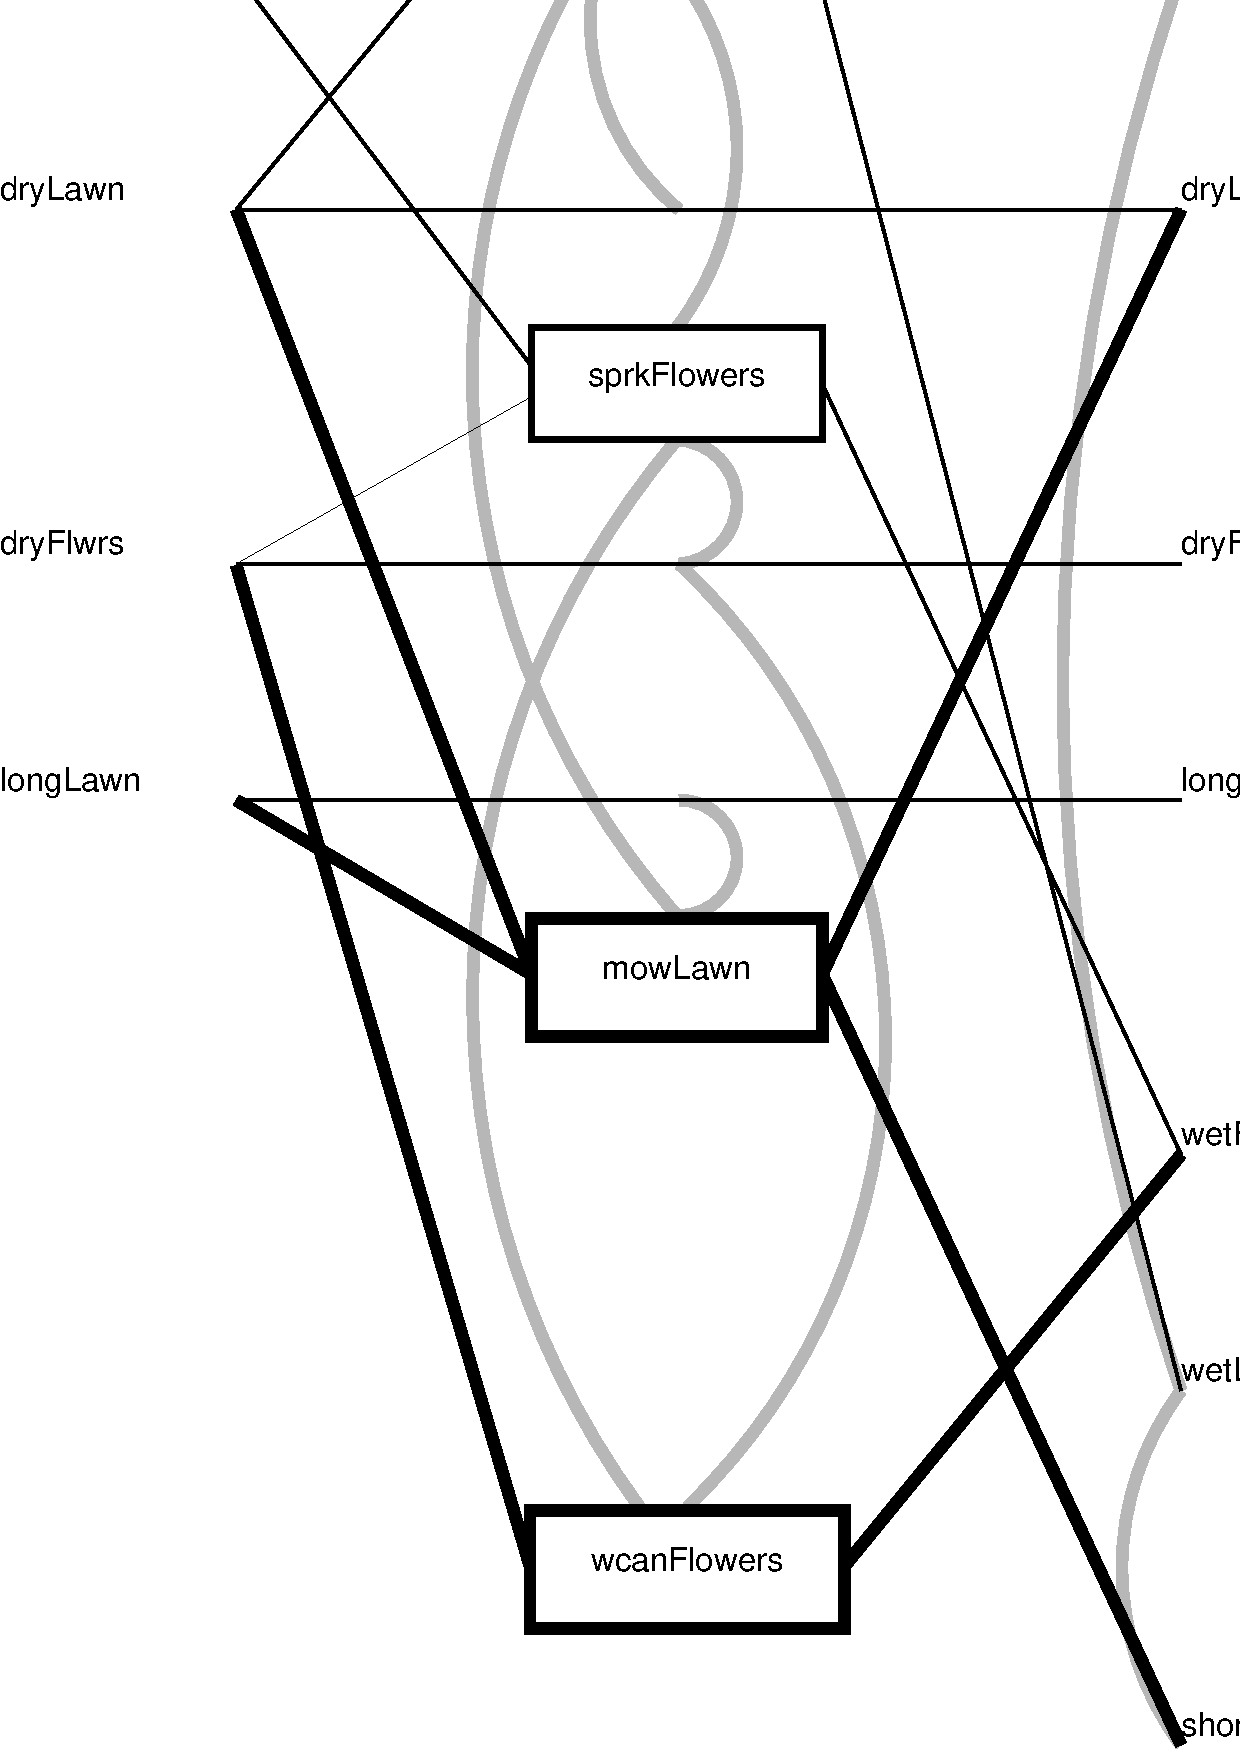
\includegraphics[scale=0.25]{non_serial.pdf}
\subsection{$S_0$}
The preconditions in the initial state of this planning graph allows all actions to be applied. Here none of the goal conditions has been satisfyed. So the graph is expanded.

\subsection{$S_1$}
Here all goalconditions has been satisfyed. There exists some mutex relations preventing all goals to be reached, the level is therefore a no-good. The most important mutex relations are: 

\begin{enumerate}

\item The actions \emph{sprkLawn} and the action \emph{mowLawn} are mutex because they both require the precondition \emph{dryLawn}.
\item The effects \emph{wetLawn} and \emph{shortLawn} are mutex because\emph{sprkLawn} and \emph{mowLawn} are mutex. 

\end{enumerate}

\subsection{$G$}
In this state, the goals are not mutex. This means that we can attempt to extract a solution. Wheter further expansion of the graph is needed, will be dertermined by the succsess or failure of the algorithm used to extract the solution.

\section{Extraction of a solution}
\subsection{Path found}
This is a list of actions applied in chronological order to reach the goal. The order of actions applied in a single action-level is not important.
\begin{itemize}
\item $A_0$
	\begin{itemize}
	\item \emph{availSprkl}
	\item \emph{mowLawn}
	\item \emph{wcanFlowers}
	\end{itemize}
\item $A_1$
	\begin{itemize}
	\item \emph{sprkLawn}
	\item \emph{wetFlwrs}
	\item \emph{shortLawn}
	\end{itemize}
\end{itemize}

\subsection{Extracting the solution}
The solution is found using a backtracking algorithm. The cost for a action is 1 and the cost for a persistence action is 0. The starting state, $G$ is at the end of the planning-graph. 
First the persistence-actions of \emph{wetFlws}, \emph{wetLawn} and \emph{shortLawn} are selected. The \emph{wetLawn} and \emph{shortLawn} in $S_1$ is mutex. One of the persistence-actions is then reverted. The \emph{wetLawn} persistent action is chosen randomly. The \emph{sprkLawn} is then applied as it is the only possible option after eliminating the persistent action.
The conditions reached so far, in level $S_1$, are:
\begin{enumerate}
	\item \emph{availSprk}
	\item \emph{dryLawn}
	\item \emph{wetFlwrs}
	\item \emph{shortLawn}
\end{enumerate}
The persistence actions of \emph{availSprkl} and \emph{dryLawn} is chosen. The \emph{sprkFlowers} action is mutex with the persistence action of \emph{availSprkl}, therefore the \emph{wcanFlowers} is chosen instead. Lastly the \emph{mowLawn} action is selected for the \emph{shortLawn} condition, wich is the only action available. The initial state has now been reached. The conditions met are:
 
\begin{enumerate}
	\item \emph{availSprkl}
	\item \emph{dryLawn}
	\item \emph{dryFlwrs}
	\item \emph{longLawn}
\end{enumerate}

Since the initial conditions have been met, the extracting algorithm has been sucessfull. There is no need for further expansion of the graph.


\end{document}



